\section{State-of-the-art in Spacecraft Modularity and Autonomous Reconfiguration}
This section explores existing cases of spacecraft modularity and reconfiguration technologies currently or previously in operation. Due to the challenges related to developing automated reconfiguration systems for space operations, there are limited existing cases of automated reconfiguration aside from the International Space Station (ISS). However, modular design principles have been integral in spacecraft development since the 1980s, notably with the introduction of the Multi-mission Modular Spacecraft (MMS).

\subsection{Multi-mission Modular Spacecraft (MMS)}

%\setlength\intextsep{0pt}
\begin{wrapfigure}{r}{0.45\textwidth}
	\centering
	\vspace{-\baselineskip}
	
	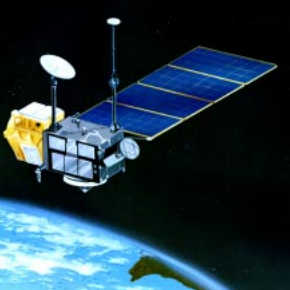
\includegraphics[width=0.45\textwidth]{mms}
	\caption{Artist rendering of the TOPEX/Poseidon mission. Image from \cite{poseidonFacts}}
	\label{MMS}
\end{wrapfigure}
 The Multi-mission Modular Spacecraft (MMS) was designed and deployed by NASA in the 1980s and 1990s \cite{Esper2005ModularAR}  with the intention of decreasing space mission costs. Intended to be recoverable/serviceable by the Space Shuttle Orbiter \cite{NasaMMS},  It is one of the first cases of modular designs seen in the space industry and has paved the way for future innovations.
 \\
 The MMS consisted of a small number of immobile modules, with the most basic deployed MMS containing only modules for altitude control, communications and data handling, and the power subsystems module \cite{Esper2005ModularAR}. 
 \\\\
 \newpage
 The MMS flew only six missions through its lifetime which was vastly different from the thirty-one expected in the 1970s \cite{Esper2005ModularAR},  it suffered limitation in the form of electronic technologies rather than mechanical restraints. NASA’s first Standard Spacecraft Computer (NSSC-1) \cite{10.1145/358234.358252}  was developed to prevent requiring an entire redesign of onboard computers for each mission, requiring only a software redesign, though this was still a heavy burden affecting the MMS’s mission flexibility. While no longer in operation as of 2006 \cite{hupp2006nasa}, the system did show cost-savings in the range of 55\% to 65\% \cite{Esper2005ModularAR}. 
 “The idea of a modular system serving many purposes was the pioneer of the leading systems within the space technology ecosystem today as it has left a lasting legacy” \cite{Esper2005ModularAR}.  In the wake of the MMS’s legacy, new design techniques were developed such as the Modular, Adaptive, Reconfigurable Systems (MARS) system-level architecture \cite{Esper2005ModularAR} that has built the foundation for modern space systems.
 
\subsection{Modular Common Spacecraft Bus (MCSB)}
\begin{wrapfigure}{r}{0.4\textwidth}
	\centering
	\vspace{-\baselineskip}
	
	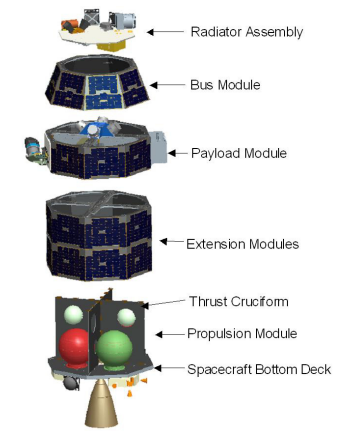
\includegraphics[width=0.4\textwidth]{ladee}
	\caption{LADEE Bus Modules from the MCSB Architecture. Image from \cite{5446989}}
	\label{LADEE}
\end{wrapfigure}

The MCSB is a fast-development, low-cost, general purpose spacecraft platform consisting of a series of 4-5 modules stacked on top of each other, each serving separate functionality \cite{tietz2009multi}. According to NASA, “the spacecraft is roughly one tenth the price of a conventional unmanned mission and could be used to land on the Moon, orbit Earth, or rendezvous with near-Earth objects.” \cite{MCSBPost} 
\\
The MCSB system received the Popular Mechanics 2014 breakthrough Award for innovation in science and technology \cite{MCSBaward} and is proving to be at the forefront of existing modular space technologies, first deployed on the Lunar Atmosphere and Dust Environment Explorer (LADEE) mission in 2013 \cite{7118961}.
\\\\
The MCSB system is an example of modularity being used to streamline and reduce costs of the initial development process of the craft, being able to carry up to 50kg of scientific equipment inside its payload module \cite{tietz2009multi}, though the end product is still a whole system that has limited in-operation service capabilities and is not capable of being reconfigured to adapt to mission requirements in-orbit.
\subsection{International Space Station}
\begin{wrapfigure}{r}{0.5\textwidth}
\centering
\vspace{-\baselineskip}

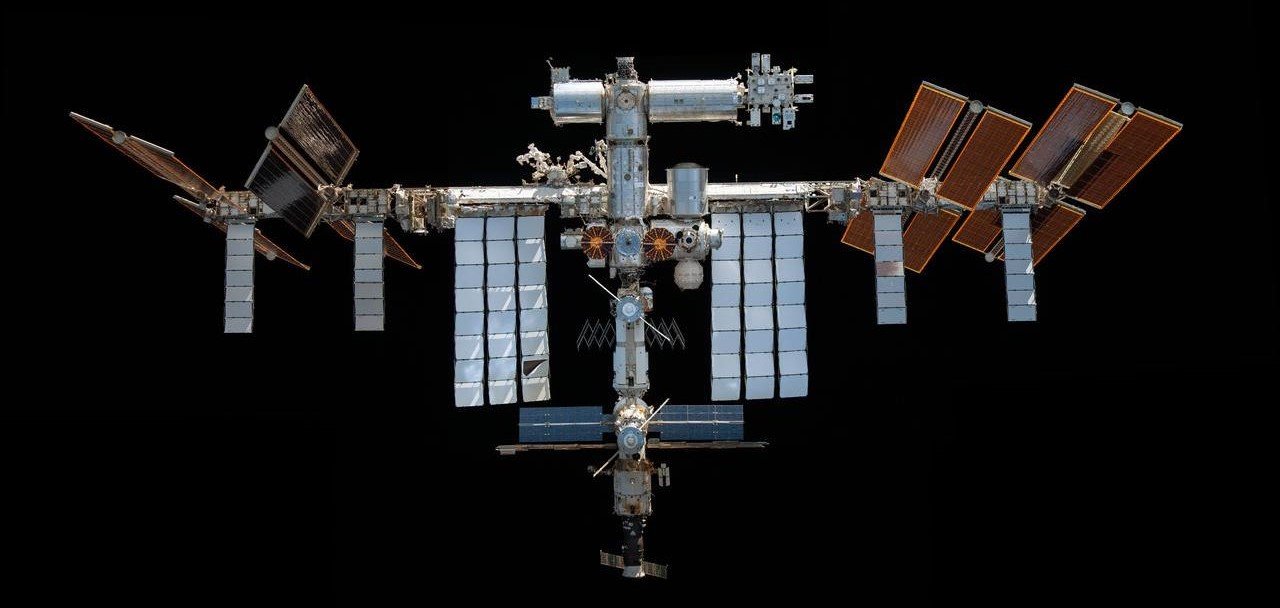
\includegraphics[width=0.5\textwidth]{iss}
\caption{The ISS pictured from the SpaceX Crew Dragon (Dec. 8, 2021). Image from \cite{issImage}}
\label{ISS}
\end{wrapfigure}
The International Space Station (ISS) seen in figure \ref{ISS} is the largest space platform ever built, created with the purpose of performing microgravity and space environment experiments. First launched in 1998\cite{shaevich2003results} and expanded through the integration of additional modules and serviced by human occupants up until its planned de-orbit in 2031 \cite{ISSdecomission}, it is a monument to advancements in the space industry.
\\\\
The ISS is capable of reconfiguration using a robotic arm and automated docking with human oversight \cite{post2019knowledge} unlike previous cases, though unsupervised automated reconfiguration is yet to be attempted due to the consequences of failure.
\\\\
Although the examples provided are not exhaustive, they encompass significant cases of modularity in the history of space exploration. Currently, automated spacecraft reconfiguration remains unimplemented in the industry. This project aims to contribute towards the future widespread adoption of automated modular reconfiguration by developing a system that can be compared with other emerging systems, aiding to identify techniques that offer the most substantial benefits. These techniques can then be utilised to create increasingly advanced reconfiguration systems for space applications.